É muito comum aparecer algum tipo de relação linear entre os dados. Nesse tipo de relação costuma-se aplicar técnicas de regressão, normalmente mínimos quadrados, para encontrar a melhor reta que representa esses dados.

Pelo alinhamento dos pontos da seção \nameref{sec:reta} e pela equação teórica (\ref{eq:resist}), fica clara a possibilidade de se aplicar uma regressão linear e, portanto, os dados continuarão os mesmos nessa seção.


\subsection{Configurações da Regressão}

    A regressão normalmente é feita pelas opções \textbf{Analysis: Fitting: Fit Linear}. Isso abre a janela de opções (figura \ref{fig:regres:opt}). Quando terminada a regressão, aparecerá uma janela perguntando para mudar de aba, mas por enquanto é melhor continuar nesta aba.

    Existem outras formas de regressão além da linear, mas essa já é o bastante para resolver todos os casos da disciplina.

    \begin{figure}[htbp]
        \centering
        \begin{subfigure}{0.60\textwidth}
            \centering
            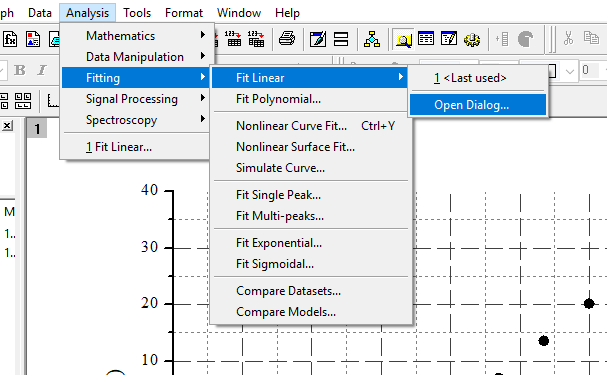
\includegraphics[width=\textwidth]{regres/1regpath.png}

            \caption{Acessando as opções de regressão}
            \label{fig:regres:path}
        \end{subfigure}
        ~
        \begin{subfigure}{0.35\textwidth}
            \centering
            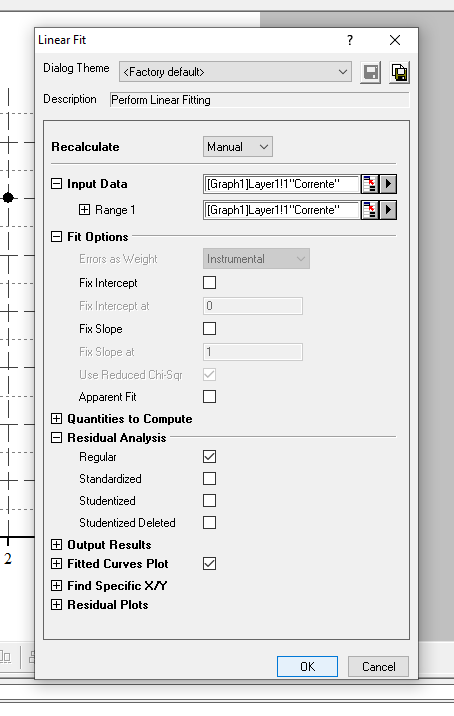
\includegraphics[width=\textwidth]{regres/2regopt.png}

            \caption{Opções de regressão}
            \label{fig:regres:opt}
        \end{subfigure}
        \caption{Configurações da regressão}
        \label{fig:regres:config}
    \end{figure}


\subsection{Tabela dos Coeficientes}

    Por padrão, os coeficientes da regressão aparecem em uma tabela como a da figura \ref{fig:regres:coefspadrao}. Ao acessar a tabela \texttt{Table1} na parte esquerda do programa, é possível modificar essa tabela. Após a modificação, é importante apertar \texttt{Update Table} para atualizar a visualização no gráfico.

    \begin{figure}[htbp]
        \centering
        \begin{subfigure}{0.45\textwidth}
            \centering
            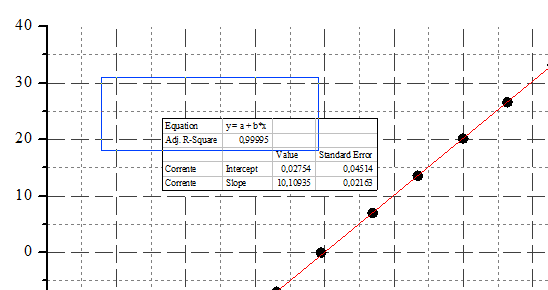
\includegraphics[width=\textwidth]{regres/4mover.png}

            \caption{Tabela padrão de coeficientes da regressão}
            \label{fig:regres:coefspadrao}
        \end{subfigure}
        ~
        \begin{subfigure}{0.50\textwidth}
            \centering
            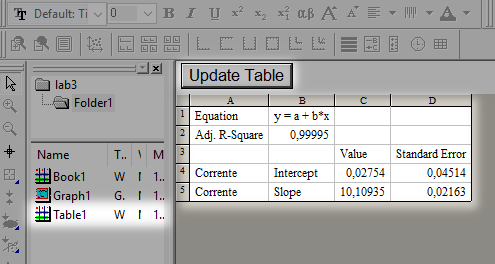
\includegraphics[width=\textwidth]{regres/5tabcoefs.png}

            \caption{Configuração da tabela de coeficientes}
            \label{fig:regres:tabcoefs}
        \end{subfigure}
        \caption{Tabela de coeficientes da regressão}
        \label{fig:regres:coefs}
    \end{figure}


\subsection{Formatação dos Coeficientes}

    Na figura \ref{fig:regres:renome2}, aparece o padrão que será seguido neste tutorial para essa tabela de coeficientes. As dimensões da tabela (figura \ref{fig:regres:tamanhos}), que mudam para cada caso, não seguirão nenhum padrão aqui.

    \begin{figure}[htbp]
        \centering
        \begin{subfigure}{0.45\textwidth}
            \centering
            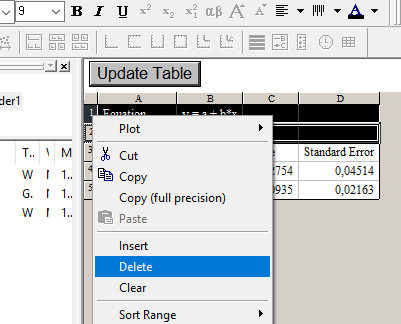
\includegraphics[width=\textwidth]{regres/6del1.png}

            \caption{Removendo as linhas superiores}
            \label{fig:regres:del1}
        \end{subfigure}
        ~
        \begin{subfigure}{0.450\textwidth}
            \centering
            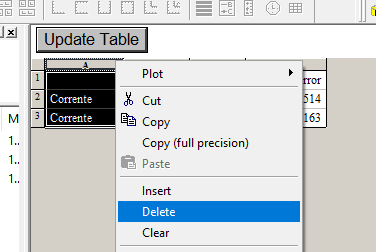
\includegraphics[width=\textwidth]{regres/7del2.png}

            \caption{Removendo as colunas de descrição}
            \label{fig:regres:del2}
        \end{subfigure}
        \caption{Reduzindo a tabela de coeficientes}
        \label{fig:regres:del}
    \end{figure}

    \begin{figure}[htbp]
        \centering
        \begin{subfigure}{0.45\textwidth}
            \centering
            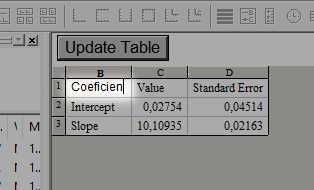
\includegraphics[width=\textwidth]{regres/8renome.png}

            \caption{Renomeando os campos}
            \label{fig:regres:renome1}
        \end{subfigure}
        ~
        \begin{subfigure}{0.450\textwidth}
            \centering
            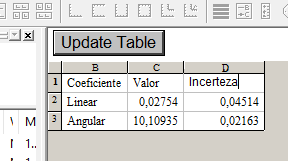
\includegraphics[width=\textwidth]{regres/9renomeado.png}

            \caption{Campos da tabela depois de renomeados}
            \label{fig:regres:renome2}
        \end{subfigure}
        \caption{Renomeando os campos da tabela de coeficientes da regressão}
        \label{fig:regres:renome}
    \end{figure}

    \begin{figure}[htbp]
        \centering
        \begin{subfigure}{0.5\textwidth}
            \centering
            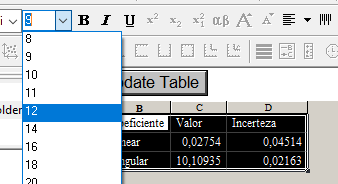
\includegraphics[width=\textwidth]{regres/10fontetam.png}

            \caption{Ajustando o tamanho da fonte}
            \label{fig:regres:fontetam}
        \end{subfigure}
        ~
        \begin{subfigure}{0.40\textwidth}
            \centering
            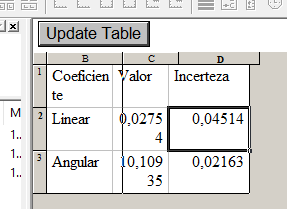
\includegraphics[width=\textwidth]{regres/11colunatam.png}

            \caption{Ajustando a largura da coluna}
            \label{fig:regres:colunatam}
        \end{subfigure}
        \caption{Ajustando as dimensões da tabela de coeficientes da regressão}
        \label{fig:regres:tamanhos}
    \end{figure}

    \begin{figure}[htbp]
        \centering
        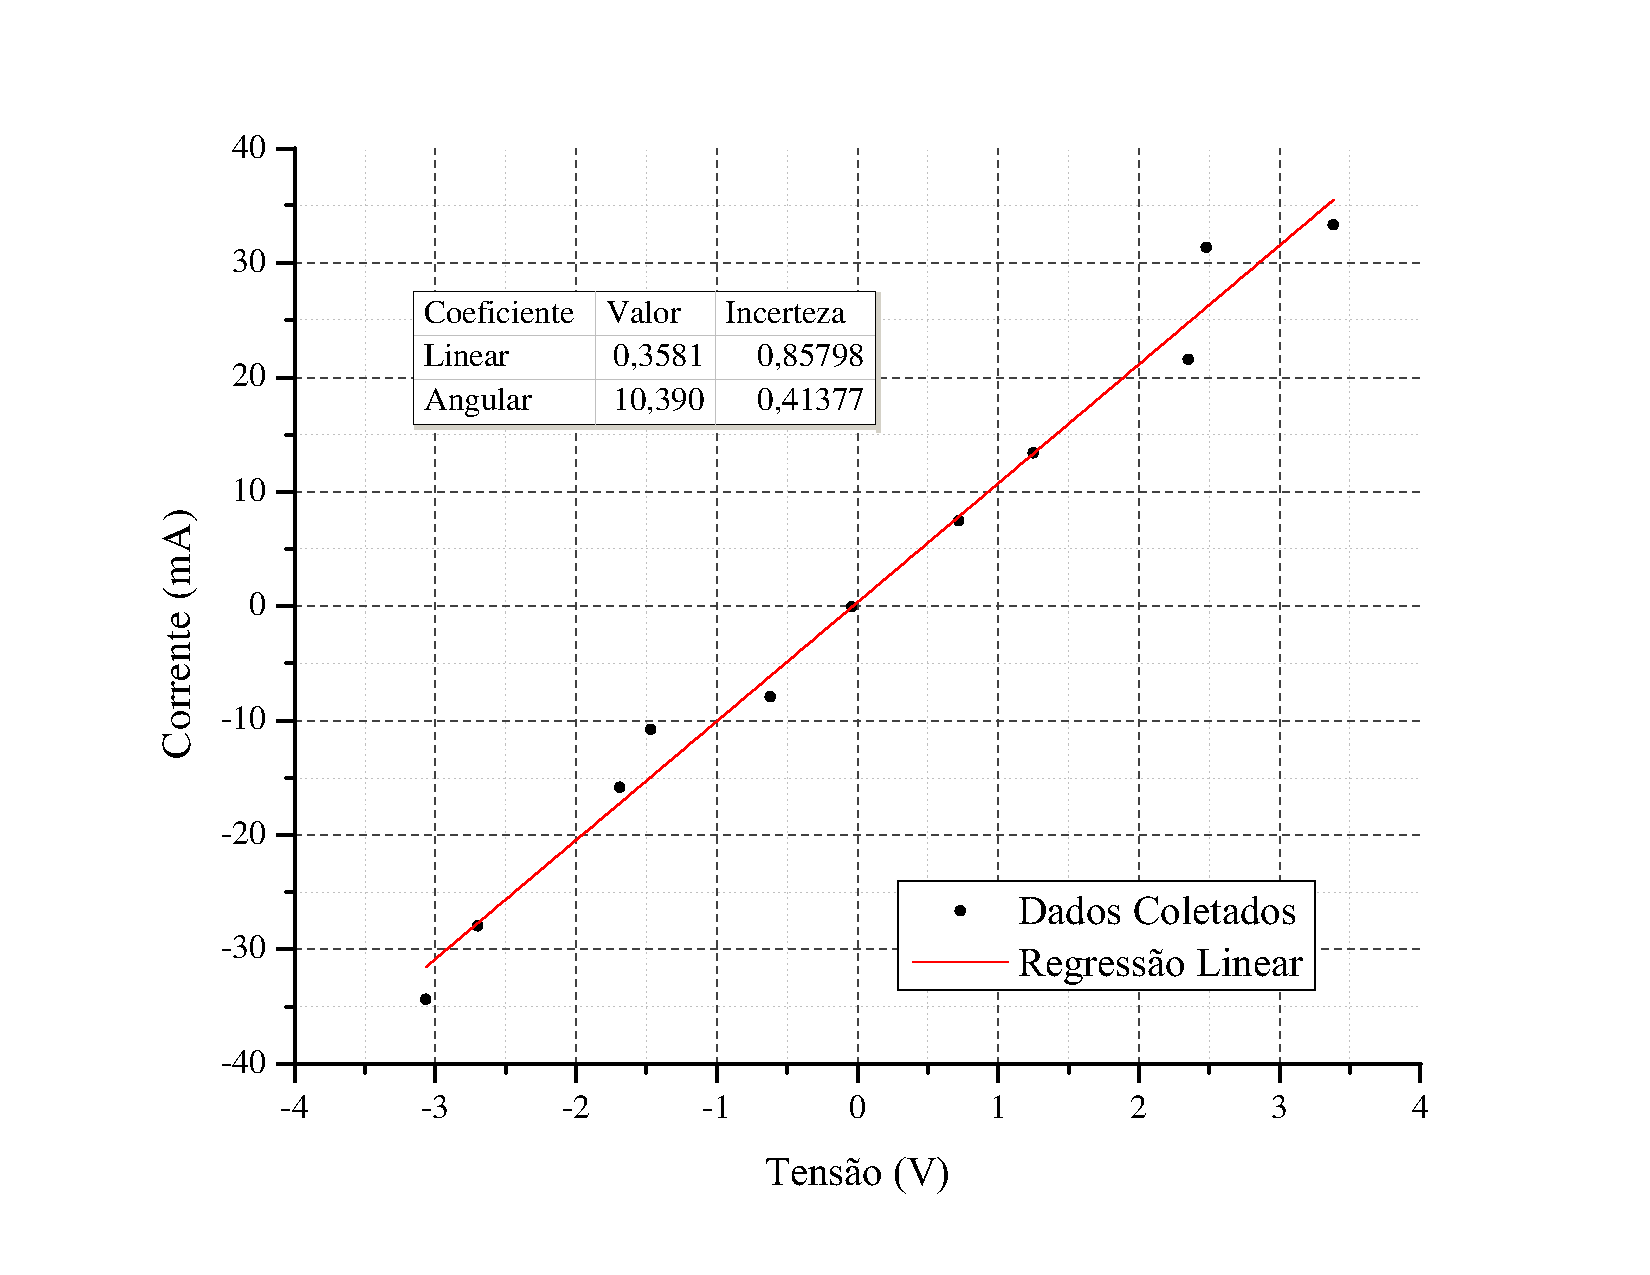
\includegraphics[width=0.8\textwidth]{regres/z1parcial.pdf}

        \caption{Exemplo de regressão linear para a relação de corrrente por tensão}
        \label{fig:regres:semifinal}
    \end{figure}


\subsection{Pontos Fora da Reta}

    Podemos ver que a regressão (figura \ref{fig:regres:semifinal}) resultou em alguns pontos que não ficaram muito próximos a reta encontradada. Esses pontos podem ser marcados para serem ignorados na regressão, como mostra a figura \ref{fig:regres:outliers}. Note que os pontos marcados passam a ser coloridos em vermelho (figura \ref{fig:regres:recalc}).

    \begin{figure}[htbp]
        \centering
        \begin{subfigure}{0.35\textwidth}
            \centering
            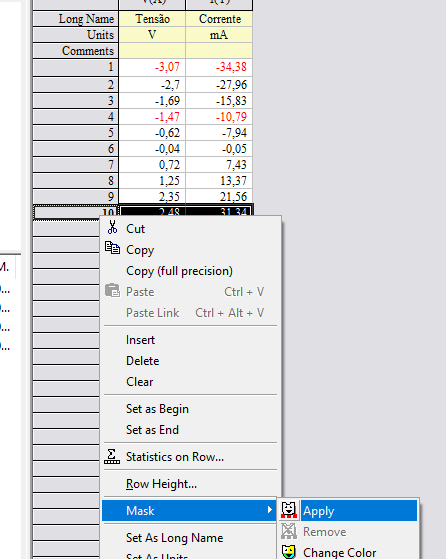
\includegraphics[width=\textwidth]{regres/12remov.png}

            \caption{Marcando os pontos a serem ignorados}
            \label{fig:regres:mask}
        \end{subfigure}
        ~
        \begin{subfigure}{0.35\textwidth}
            \centering
            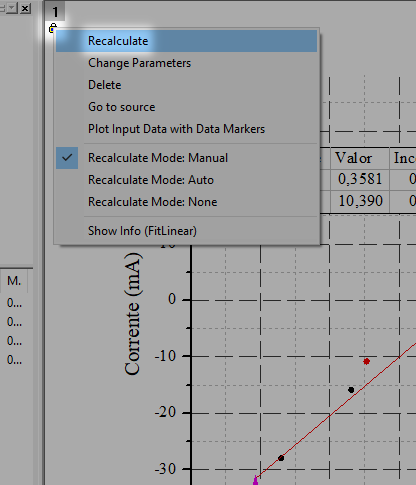
\includegraphics[width=\textwidth]{regres/13recalc.png}

            \caption{Recalculando os coeficientes da regressão}
            \label{fig:regres:recalc}
        \end{subfigure}
        \caption{Removendo pontos selecionados da regressão}
        \label{fig:regres:outliers}
    \end{figure}


\subsection{Resultado}

    \begin{figure}[htbp]
        \centering
        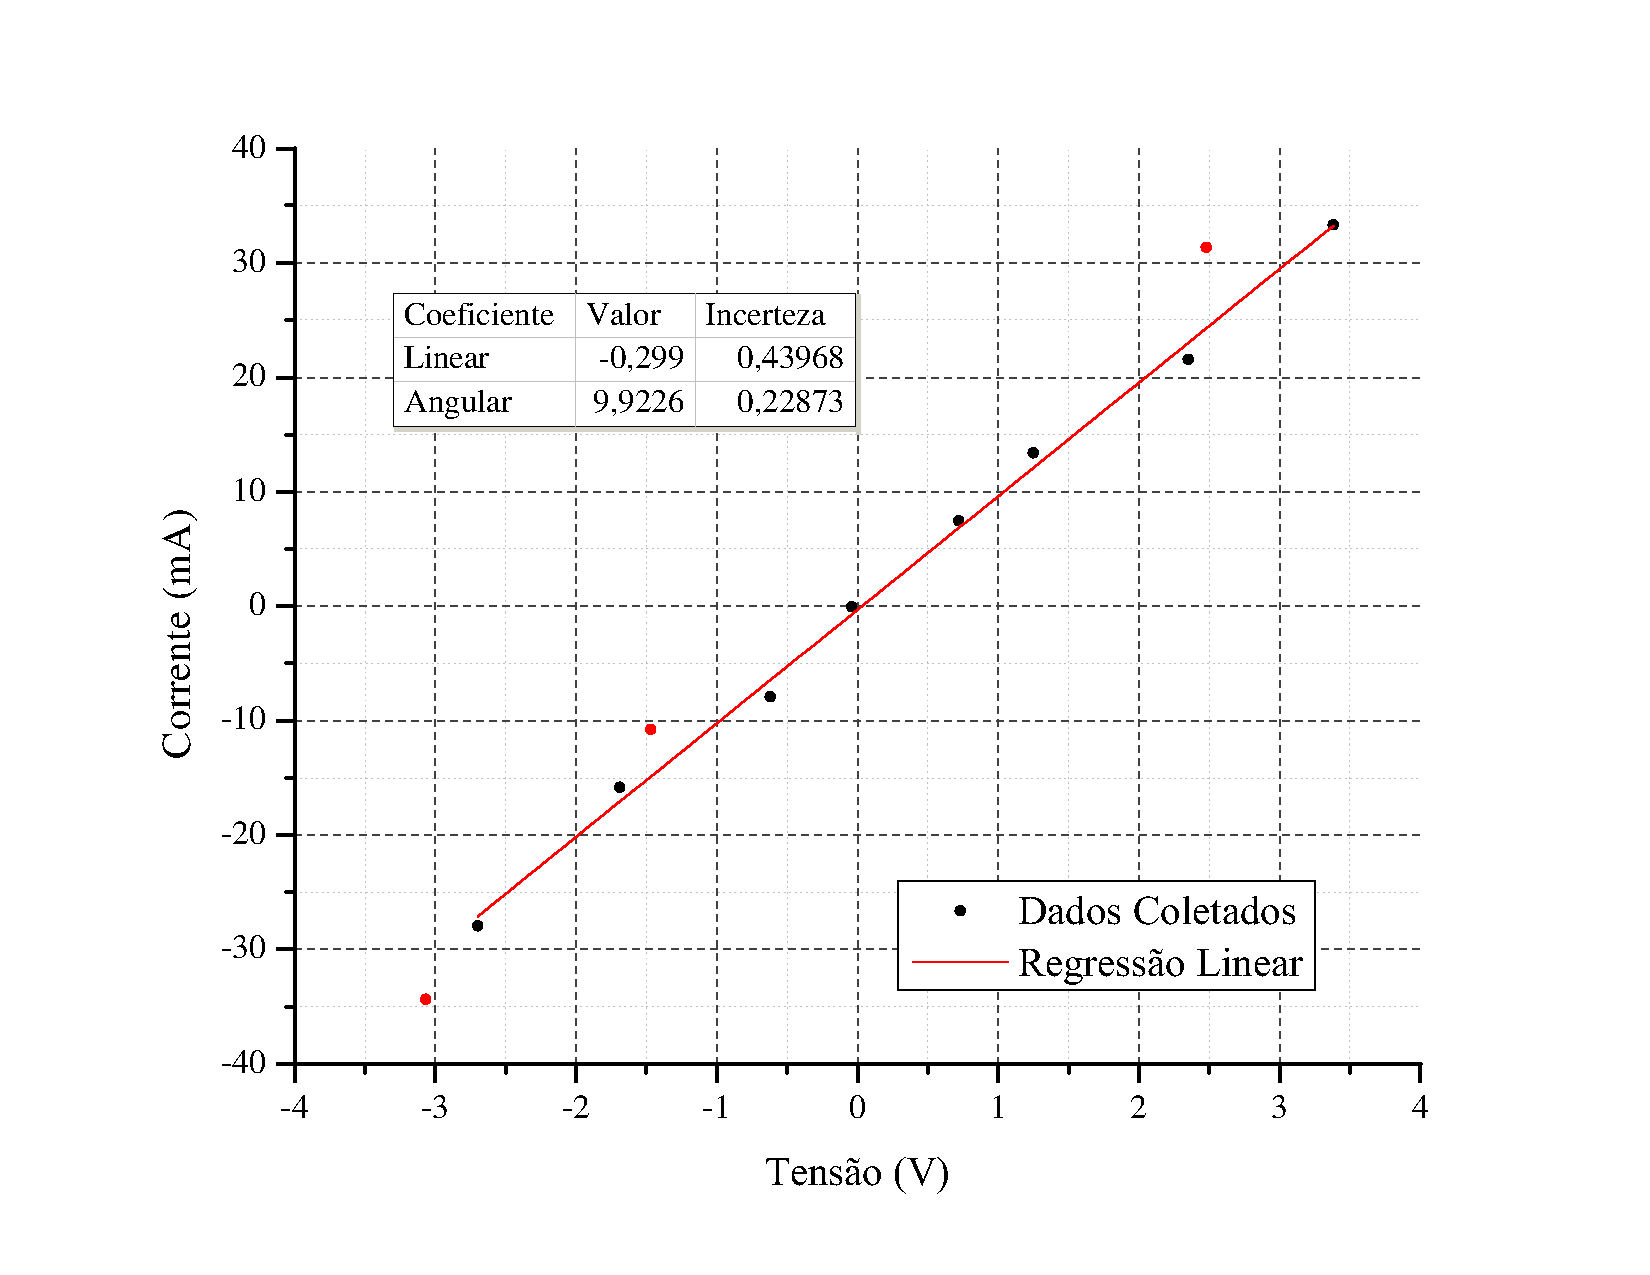
\includegraphics[width=0.8\textwidth]{regres/z2final.pdf}

        \caption{Exemplo de regressão linear com pontos ignorados}
        \label{fig:regres:final}
    \end{figure}

    Observando o resultado na figura \ref{fig:regres:final}, a nova regressão com os pontos ignorados obteve uma redução significativa na incerteza dos coeficientes. Isso indica que a remoção de \textit{outliers} é um passo importante na medição, mas deve ser feito com cuidado. A retirada de pontos válidos para a regressão pode reduzir ambas a precisão e a exatidão dos resultados, pela maneira como o cálculo da regressão é feito.
